\documentclass[12pt]{article}

\usepackage{fullpage}
\usepackage{graphicx, rotating, booktabs} 
\usepackage{times} 
\usepackage{natbib} 
\usepackage{indentfirst} 
\usepackage{setspace}
\usepackage{grffile} 
\usepackage{hyperref}
\usepackage{adjustbox}
\usepackage{amsmath}
\usepackage{siunitx}
\usepackage{multirow}
\setcitestyle{aysep{}}


\singlespace
\title{\textbf{Elite Cues and Public Attitudes Towards Military Alliances}}
\author{Joshua Alley \\
Postdoctoral Research Associate \\
University of Virginia.\thanks{Thanks to Erik Lin-Greenberg, Philip Potter, Justin Schon and Todd Sechser, as well as participants in the Democratic Statecraft Lab Research incubator, the Lansing B. Lee/Bankard Seminar in Global Politics, 2020 Annual Meeting of the Peace Science Society and 2021 Meeting of the International Studies Association for helpful comments. This project was reviewed by the University of Virginia IRB (Protocol 3866) and preregistration files for this study are hosted in an OSF repository at https://osf.io/g28zs.} \\
jkalley@virginia.edu
}
\date{}

\bibliographystyle{apsr}

\begin{document}

\maketitle 

\doublespace 

\begin{abstract}
What drives public support or opposition to military alliances in the United States? 
Answering this question requires identifying who leads whom between elite cues and public opinion.  
To address this longstanding puzzle, I demarcate the extent of elite influence on public alliance attitudes by explaining how partisanship and foreign policy dispositions shape individual responses to elite cues and alliance characteristics. 
I then use two conjoint survey experiments to examine the roots of public attitudes towards forming and maintaining international alliances.  
I find that elites can lead most of the electorate, but subsets of both major parties hold rigid attitudes. 
These fixed attitudes have a partisan asymmetry, as staunch alliance supporters in the Democratic party and consistent alliance skeptics in the Republican party both ignore elite cues.  
Elites lead public opinion towards military alliances, but partisanship and foreign policy dispositions constrain and shape their impact.  
\end{abstract}


\newpage 


\section{Introduction}

% lay out the question
What determines U.S. public opinion towards military alliances? 
Despite the importance of public attitudes for forming and upholding U.S. alliances, we do not know why the public supports or opposes alliance commitments. 
Most evidence on this question comes from opinion polls measuring public sentiment towards alliances like the North Atlantic Treaty Organization (NATO).
These polls provide useful data, but they do not explain why individuals express particular opinions. 


% puzzle
Descriptive polling data has limited explanatory power because alliance attitudes are subject to the longstanding puzzle of who leads whom in public opinion on foreign policy.\footnote{This article considers the leading or following question for Trump and NATO: \url{https://fivethirtyeight.com/features/is-trump-fueling-republicans-concerns-about-nato-or-echoing-them/}}
On the one hand, elites have ample opportunity to lead public opinion on alliances, given limited public information and interest in foreign policy \citep{Canes-Wrone2006, BaumPotter2008, Druckman2014}.
On the other, leaders often follow public attitudes \citep{Barberaetal2019, HagerHilbig2020}.
Alliance politics have low public salience, which likely increases elite influence. 
But even when the public pays little attention to international affairs, their opinions have consistency and structure \citep{Holsti1992, PageShapiro1992}.
Individual foreign policy dispositions \citep{KertzerZeitzoff2017} could establish alliance attitudes for leaders to follow.
For instance, Republicans have a history of isolationism and skepticism towards alliances that party elites may follow. 


% contribution
I explore the roots of U.S. alliance attitudes by examining how foreign policy dispositions and partisanship change individual responses to elite cues and alliance characteristics.
Whether elites lead or follow public opinion depends on how elite cues impact individuals with different predispositions towards alliances from isolationism and militant assertiveness.  
Isolationists are skeptical of alliances, while hawks often back alliance participation. 
If elite cues encourage isolationists to support alliances and hawks to oppose alliances, elites lead alliance attitudes. 
But if elite cues have no impact or only move individuals in ways that match their predispositions, elites are more likely to follow public opinion.


% Assess w/ a survey experiment
To provide causal evidence on the sources of public opinion towards alliances, I use two conjoint survey experiments.
Conjoint experiments allow me to randomize many alliance characteristics and elite cues \citep{Hainmuelleretal2014}.
Unlike in observational data, in an experiment that randomly assigns elite cues, I can leverage information on foreign policy dispositions within parties to distinguish who leads and who follows. 
The first experiment scrutinizes attitudes towards alliance formation, while the second addresses alliance maintenance. 


% findings: fix this para up! 
In two nationally representative samples, I find that while most individuals follow co-partisan elite cues regardless of their foreign policy dispositions, the strongest alliance supporters in the Democratic party have rigid alliance attitudes, as do staunch alliance skeptics in the Republican party. 
The base from which elite cues move alliance attitudes also depends on partisanship and foreign policy dispositions.
Elite cues thus exert broad influence, but their impact depends on partisanship, hawkishness and isolationism, which create substantial variation in alliance attitudes.
How elites change alliance attitudes depends on where those attitudes start.  


There is a partisan divide in rigid alliance attitudes.
Hawkish and isolationist Democrats are robust alliance supporters.
Dovish and isolationist Republicans are committed alliance skeptics. 
Therefore, Republicans can lead the most likely alliance supporters in their party, while Democrats can lead relative alliance skeptics. 
If elected leaders follow the strongest alliance attitudes in their party, they will polarize the rest of the electorate. 


% partisan differences in democracy, region
A few alliance characteristics also impact public attitudes. 
Democrats and most Republicans prefer alliances with other democracies to supporting nondemocracies. 
Issue linkages increase public support for alliance participation, while high financial costs reduce support for alliance maintenance. 
Some Republicans express strong regional preferences, with minimal interest in alliances with African and Middle Eastern states. 


% differences between formation and mainteance
I also find a gap between public support for alliance formation and maintenance.
Even with elite opposition, upholding existing alliances almost always retains majority support. 
In alliance formation, elite cues determine whether a new treaty has majority or minority support. 
Therefore, elites have more influence over adding new alliance obligations than changing existing commitments. 


% Importance part 1: public opinion undergirds alliance com in democ
In addition to providing new insight into the debate over who leads whom, there are three reasons that understanding U.S. public opinion towards alliances is worthwhile. 
To start, public opinion is central to debates over whether democracies make more reliable commitments than other states.\footnote{Public opinion is important, but it is not deterministic. \citet{Kreps2010} notes that public disapproval may not hinder coalition warfare, especially when elite consensus favors fighting.} 
If public opinion towards alliances is indifferent to elite cues, stable attitudes and reliable commitments follow \citep{Gaubatz1996}.
If elite cues drive public opinion, then public attitudes can shift quickly, leading to cycles that hinder democratic reliability \citep{GartzkeGleditsch2004}.
NATO leaders often worried that changing public attitudes would undermine the alliance \citep{Sayle2019}.  
Some observers feared that Donald Trump's rhetoric would undermine domestic support for alliances.
Yet U.S. public approval of alliances like NATO changed little during the Trump administration \citep{PewNATO2020}. 


% importance part 2: practical relevance- US role in world. 
Why the public supports or opposes alliances also speaks to the consequences of a prominent scholarly and policy debate. 
Two competing visions of U.S. foreign policy depend on alliances. 
One view believes that the United States should reduce its alliance commitments to pursue a restrained grand strategy \citep{Preble2009, Posen2014}.
The other argues that continued deep engagement through alliances is the best way to promote U.S. security and prosperity \citep{Brooksetal2013, BrandsFeaver2017}. 
If elite cues drive public opinion, leaders will face fewer public constraints on implementing these views. 


% importance part 3: WHY support international cooperation, not just consequences of international institutions
In addition to its practical importance, this study fills a gap in international institutions scholarship. 
Scholars are more likely to study how international institutions affect public attitudes (e.g. \citep{KayaWalker2014, Greenhill2020}), than scrutinize the sources of public attitudes towards international institutions themselves. 
Other studies use observational survey data to examine public opinion towards international cooperation in multilateral financial institutions \citep{Edwards2009} or the United Nations \citep{Torgler2008, DellmuthTallberg2015}. 
That leaves limited causal evidence on why individuals hold particular alliance attitudes.
In one study of public opinion and military alliances, \citet{TomzWeeks2021} address a different question by showing that the presence of an alliance increases public support for foreign military intervention. 
\citet{Chuetal2021} explore how values and interest based elite cues shape public attitudes towards alliance maintenance. 
I build on these works with more general experiments on alliance formation and maintenance that clarify the reach of elite cues and examine many alliance characteristics. 


% Implications
The findings that elites have substantial influence on public attitudes towards alliances, but some individuals hold rigid opinions due to their partisanship and foreign policy disposition thus have important implications for the future of U.S. alliance politics. 
Although elite cues affect public support for U.S. alliances, one group of elites alone cannot produce majority opposition to existing treaties, because alliance maintenance commands substantial support.
Bipartisan opposition to alliances could reduce public support enough for leaders to withdraw from an alliance with little public disapproval, however.  
Unlike existing treaties, public support for new alliance commitments is vulnerable to elite criticism. 
Whether elites in the two major parties follow the contradictory fixed attitudes in their parties will shape domestic support for U.S. international engagement through alliances.

% Try it w/o the plan of paper for flow. 


\section{Who Leads Whom in Alliance Attitudes?}


Public opinion molds democratic foreign policy and alliance politics in several ways.
First, it affects military intervention decisions \citep{Tomzetal2020, LinGreenberg2021}. 
In democracies, anticipation of paying public audience costs for treaty violation encourages limited promises of military support \citep{Chibaetal2015, FjelstulReiter2019}. 
Moreover, public attitudes are central to disputes about the reliability of democratic alliances \citep{Gaubatz1996, GartzkeGleditsch2004}. 
Policymakers also pay careful attention to public support for alliances \citep{Sayle2019}. 


% NATO example to bring out the puzzle
In addition to its importance, pubic opinion towards military alliances varies. 
\autoref{fig:nato-op-time} plots the percentage of respondents supporting NATO in 59 surveys from 1974 to 2020.\footnote{These surveys ask respondents to assess NATO in many ways. I consider favorable opinions, feeling thermometer ratings of 50 or higher, and support for increasing or maintaining U.S. commitment as indicators of support for NATO.} 
Most surveys show majority support for NATO, but public support has fallen since 2000.  


\begin{figure}
	\centering
		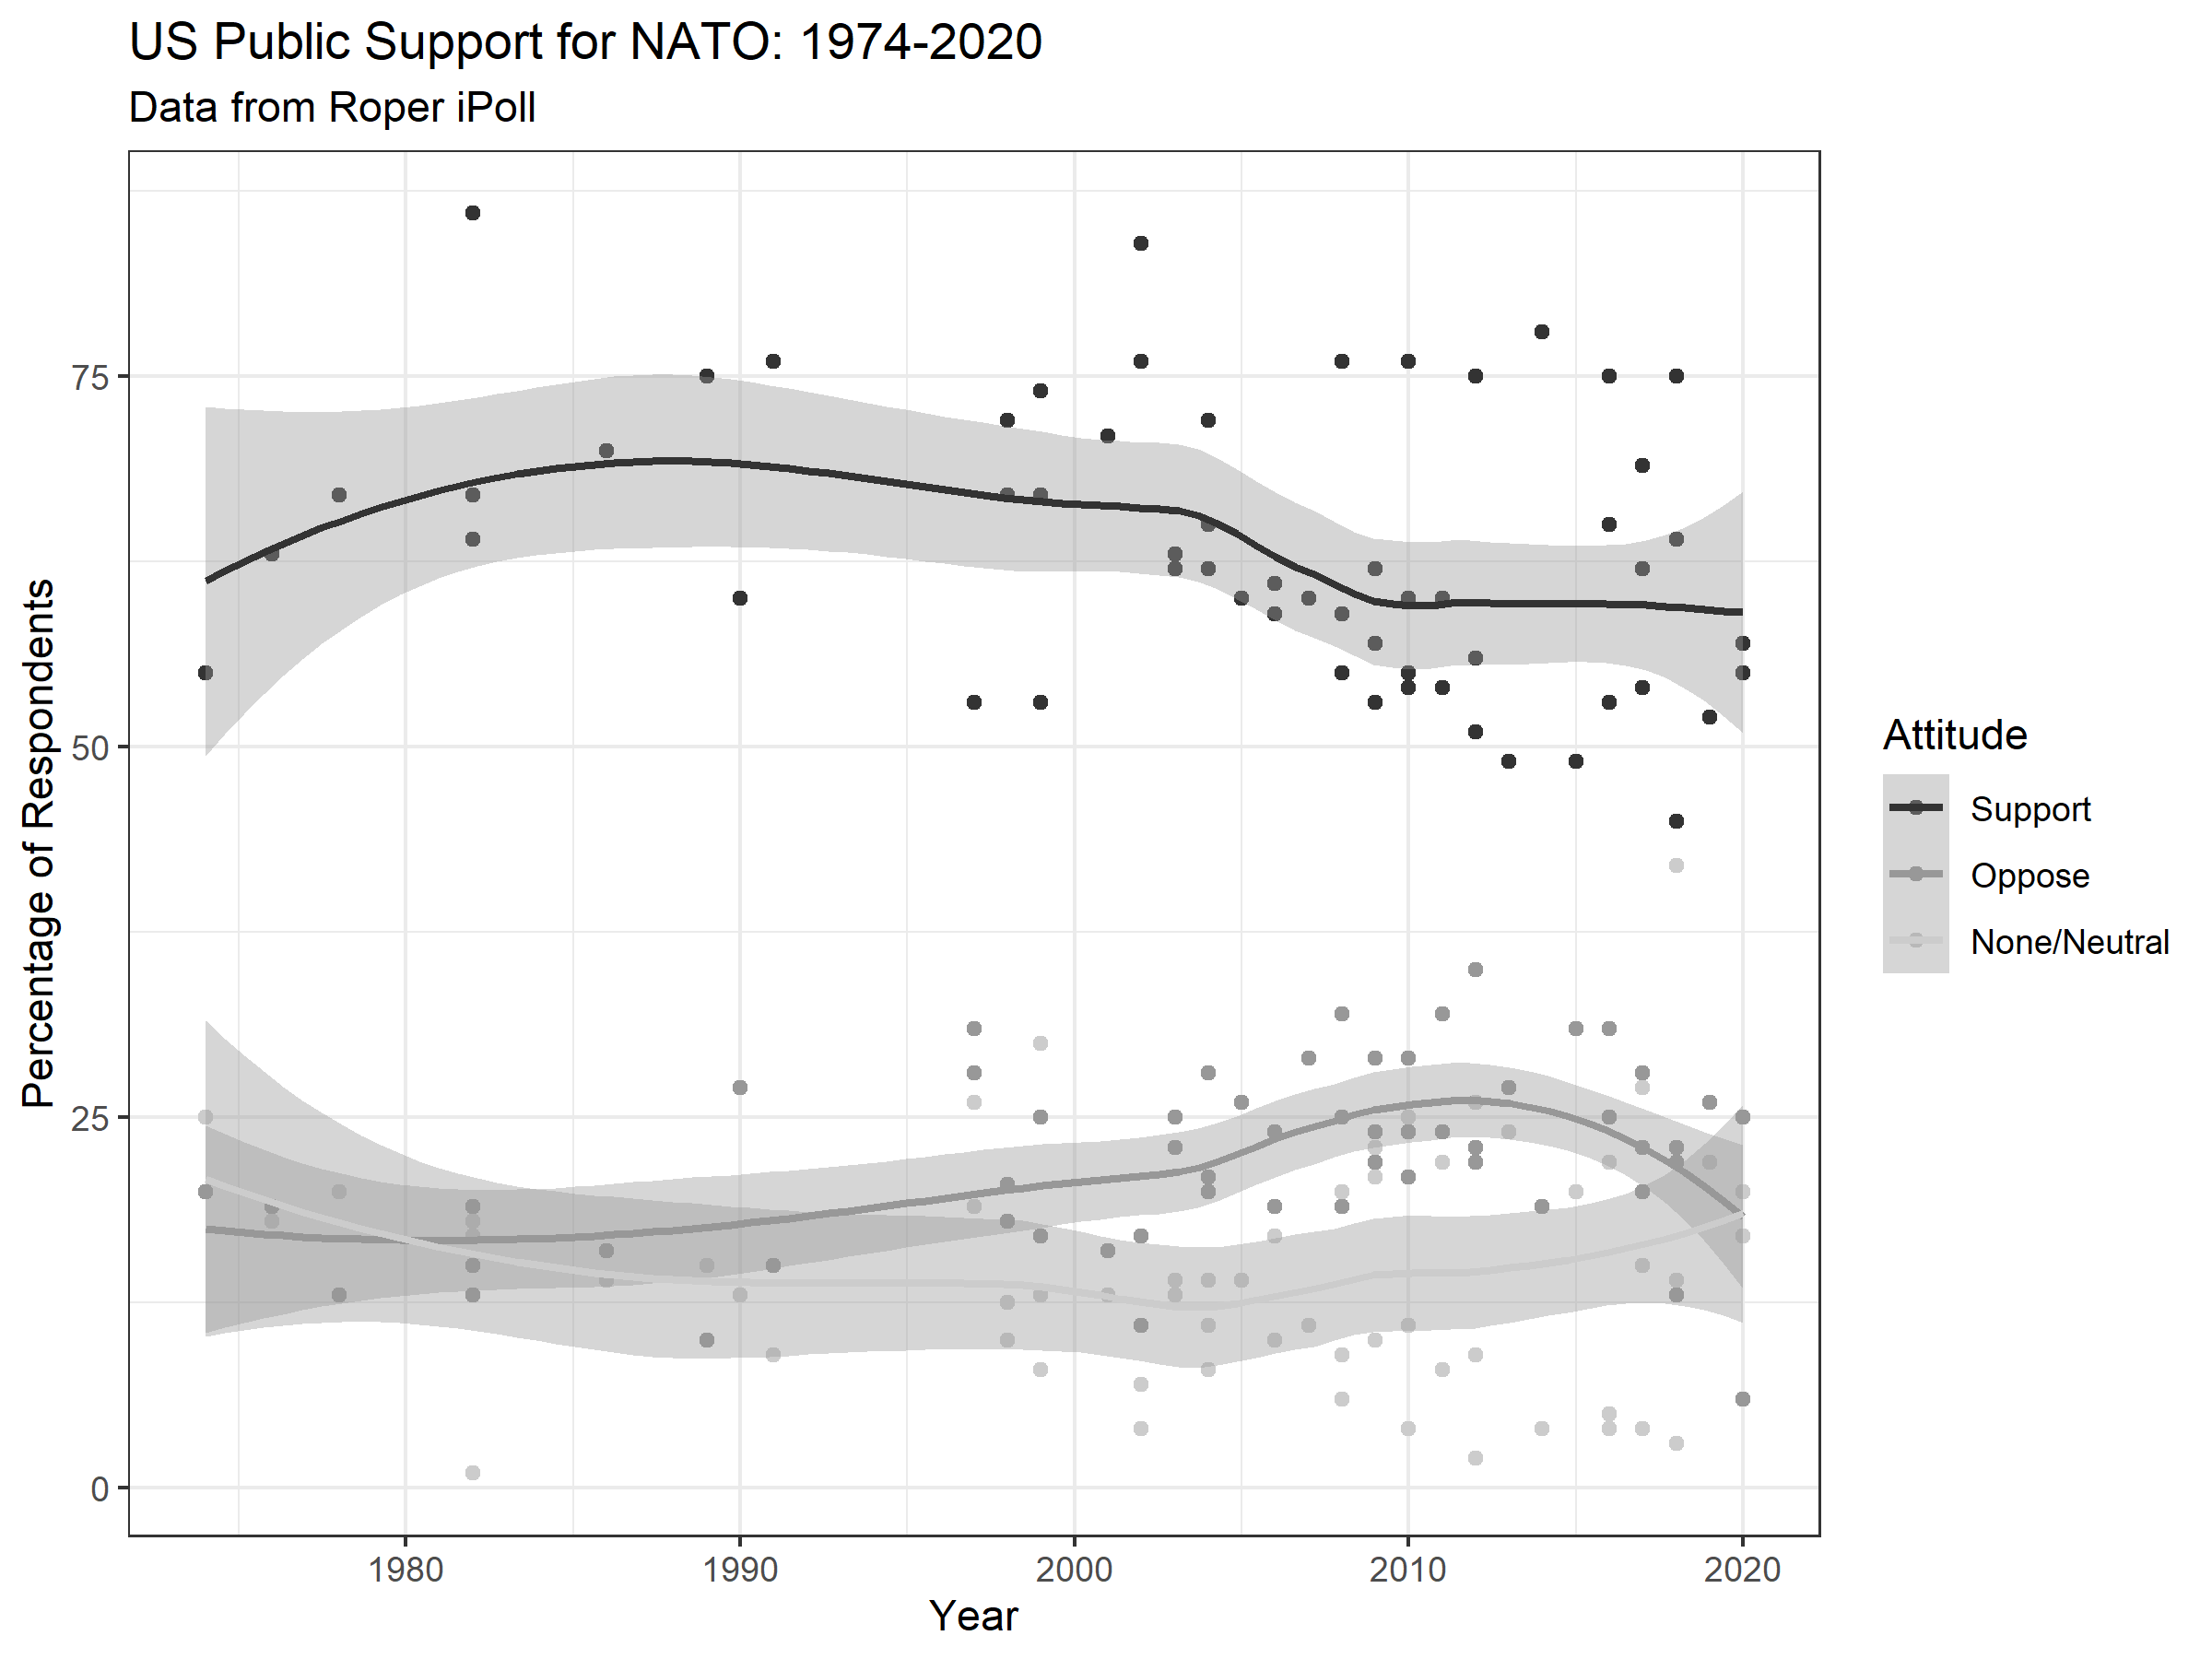
\includegraphics[width=0.95\textwidth]{../figures/nato-op-time.png}
	\caption{US public support for NATO from 1974 to 2020. Each point marks a unique poll, and colors differentiate the percentages of respondents that expressed support, opposition or neutral/no opinion of NATO. Loess lines estimate the average support for each group in every year. Topline data from the Roper Center's iPoll database.}
	\label{fig:nato-op-time}
\end{figure}



Observed alliance attitudes like those in \autoref{fig:nato-op-time} are subject to a longstanding puzzle in public opinion on foreign policy--- who leads whom? 
In this case, does public support for NATO lead or follow elite cues? 
Put differently, if we observe elite support for alliances and high public support, it is unclear if public attitudes follow elite cues or if established public attitudes drive elite cues. 
Both perspectives offer plausible models. 


Evidence on whether elites lead or follow public opinion is divided, as the following examples show.
Some suggest that elites are more likely to lead public opinion. 
\citet{Canes-Wrone2006} finds that U.S. Presidents rarely follow public preferences if they disagree, and have ample freedom to lead foreign policy attitudes. 
\citet{JacobsShapiro2000} argue that elites track public opinion to manipulate it, not conform to it. 
\citet{Kreps2010} notes that public disapproval did not constrain participation in NATO's International Security Assistance Force in Afghanistan. 
Moreover, foreign policy is a secondary concern for many voters, so elite foreign policy views and rhetoric can diverge from public attitudes with few political repercussions \citep{BusbyMonten2012}. 


Other findings suggest that elites conform their rhetoric and policy stances to public opinion. 
\citet{Barberaetal2019} use social media data to show that legislators are more likely to follow than lead public opinion, including on some foreign policy issues. 
\citet{HagerHilbig2020} find that exposure to public opinion research moves speech and policy positions by German politicians closer to majority opinion. 
\citet{GuisingerSaunders2017} claim that for issues with low partisan polarization, information effects dominate public opinion, though elite cues matter more for polarized issues like cap and trade schemes. 
\citet{Haesebrouck2019} uncovers little evidence that European elites led their public to support military interventions in Libya and the Islamic State. 
\citet{Bechteletal2015} find that elite cues and frames led Swiss individuals, especially those with low knowledge, to reinforce their prior immigration attitudes. 
Even military elites with no electoral concerns shape their recommendations in response to public opinion \citep{LinGreenberg2021}. 



Alliance attitudes are subject to this puzzle or who leads whom. 
On the one hand, limited public information about alliances will increase elite influence \citep{Druckman2001}. 
On the other, the public opinion towards alliances may depend on individual concerns, including foreign policy dispositions, as these intuitions about international affairs provide consistent heuristics even with limited information \citep{Herrmannetal2009, KertzerZeitzoff2017}.
A combination of the two is possible, and some alliance attitudes may be more plastic than others. 
\citet{PageShapiro1992} note that public opinion is broadly consistent and rational, and changes in predictable ways in response to information from multiple sources, including elite cues. 


Understanding alliance attitudes therefore speaks to a fundamental debate about public opinion on foreign policy.  
In the following, I explain how partisanship and foreign policy dispositions provide leverage to understand who leads whom.
First, I outline how elite cues lead public opinion. 


\subsection{Elite Cues} 
% Framing/elite leading
% Debate over leading/pandering

Elite cues are a plausible determinant of alliance attitudes. 
Under this general model the public follows trusted elites in forming their opinion, so elite portrayals of alliances bolster or undermine public support.
Thus, public opinion towards alliances permeates down from the top and is endogenous to elite views \citep{Druckman2014}.
There is substantial evidence that elites influence public foreign policy attitudes \citep{BaumPotter2008}. 
The media often convey elite cues and frames.
Social media may further amplify elite influence \citep{BaumPotter2019}.   


Information shortcomings make individuals more responsive to elite framing and cues \citep{Druckman2001, Peterson2017} and the public has limited foreign policy information \citep{BaumPotter2008}.
Furthermore, alliance politics has low salience within foreign policy. 
Alliances are less prominent than international conflict, which is the most common subject in studies of foreign policy opinions. 
Therefore, elite support or opposition could shape alliance attitudes because individuals rely on trusted elites in an issue environment with little alternative information. 


% cue-giver matters 
Multiple elites can give public cues about alliances.
Elected officials, diplomats and military leaders all participate in alliance politics.
The public visibility and influence of elected leaders is well-established.  
Cues from military leaders can shape public opinion about the use of force \citep{Golbyetal2018}, so military endorsements may also move alliance attitudes. 
Diplomatic elites are high profile domain experts. 
Public perceptions that military leaders and diplomats are well-informed about alliances will likely increase their influence. 


% highlight partisanship 
Partisanship further shapes elite influence.
Under partisan polarization, individuals distrust and discount messages from out-partisan elites. 
Conversely, trust makes cues from co-partisan elites more influential \citep{Druckmanetal2013}. 


% summary 
In an elite cues model, support for alliances by trusted elites should increase individual support for alliances, and elite opposition will reduce support.  
As a result, unified elite cues will have a large impact.
For example, \citet{Berinsky2007} finds that unified elite support for war leads to robust public support. 


% transition paragraph: scope of influence
Elite cues are a straightforward and compelling explanation of alliance attitudes.
Even information about alliance characteristics like allied democracy or military spending likely reaches the public through elite sources. 
When they receive elite messages, individuals also hold prior attachments, intuitions and beliefs, however.
Partisanship and individual foreign policy dispositions could modify how rigid or plastic alliance attitudes are in the face of elite cues. 


\subsection{Foreign Policy Dispositions}


% Overview para
Foreign policy dispositions shape individual perceptions of the value of international cooperation. 
These individual concerns have two consequences for alliance attitudes. 
First, they establish individuals' baseline alliance support, or willingness to back alliances in general.\footnote{Another way to think of baseline support is an individual disposition to support an average or typical alliance.} 
Second, individual concerns might change individual responses to elite cues and particular alliance characteristics. 


% foreign policy disposition
Many individuals have stable intuitions about international politics. 
These principles shape how people respond to foreign policy decisions, such as backing down from military intervention promises \citep{KertzerBrutger2016}. 
Militant assertiveness and internationalism are two key foreign policy dispositions \citep{Herrmannetal1999}.  
These principles change what individuals think of alliance commitments. 


% internationalists more likely
% Define internationalism  
Internationalism is an inclination to engage with other countries and contribute to international endeavors. 
Internationalist respondents support American engagement in foreign affairs and will favor alliance commitments. 
Conversely, isolationists are skeptical of international institutions and cooperation, dislike foreign involvement and prioritize domestic affairs \citep{Kertzer2013}. 
As a result, isolationists should be skeptical of alliances and especially opposed to alliances with substantial financial cost or additional obligations. 


% militant assertiveness 
Militant assertiveness increases support for alliance participation. 
Hawkish individuals are more willing to use force to address international problems. 
Although alliances are a cooperative institution, they also aggregate military capability \citep{FordhamPoast2014} and obligate members to fight.
Hawks value capability aggregation through alliances and are willing to hazard foreign wars.  
Dovish individuals are skeptical of using military force in general.
This makes them less likely to support military alliances that commit their country to fight.  


\subsection{Partisanship}

% partisanship 
Militant assertiveness and internationalism are connected to partisanship, as they vary across and within the Democratic and Republican parties. 
Conservatives in the United States have a longstanding history of isolationist sentiment \citep{Kupchan2020}.
As a result, many Republicans are skeptical of international engagement and alliances. 
Republicans are more hawkish than Democrats as well, however \citep{Gries2014}. 


Party identification also connects elite cues and individual concerns by determining whose cues matter.
Individuals look to cues from trusted elites, and partisanship is a straightforward heuristic for who to trust. 
Because partisanship reflects foreign policy dispositions and connects to elite cues, it has a crucial role in alliance attitudes. 


% limits 
Understanding alliance attitudes thus requires careful attention to elite cues, partisanship and foreign policy dispositions. 
Although elite cues are likely influential, the extent of elite influence is unclear because partisanship changes individual perceptions of elites and is correlated with foreign policy dispositions like isolationism and militant assertiveness that shape individual dispositions towards alliances. 
Perhaps Republican leaders' opposition to alliances does not decrease Republican support for alliances, it simply reflects conservative isolationism, for instance. 


% partisanship puzzle
%At the same time, because partisanship and foreign policy dispositions are correlated, disentangling them is essential. 
%In particular, any analysis must establish whether partisan differences in alliance attitudes are the result of party affiliation or foreign policy attitudes that are correlated with partisanship. 
%To do this, I will compare the alliance attitudes of Democrats and Republicans with similar foreign policy dispositions. 
%If Republicans and Democrats with similar foreign policy dispositions hold distinct alliance attitudes, this implies that partisanship has some influence. 


\subsection{Who Leads Whom?}


% how distinguished
To assess elite leadership, I examine how elite cues impact Democrats and Republicans with different predispositions towards alliances.
Individual partisanship, militant assertiveness and isolationism create distinct inclinations to back or oppose alliances. 
These inclinations set a baseline for alliance attitudes. 
How elite cues move attitudes relative to baseline opinions provides leverage on the question of who leads whom. 


% explain: isolation
For elites to lead, their cues should change opinion regardless of individual predispositions to support or oppose alliance participation. 
If elites lead public opinion, elite support will increase support for alliance participation even among isolationists. 
Similarly, if elite opposition reduces support among hawkish individuals who would otherwise support an alliance, elite cues lead public opinion. 


% explain: hawks 
If elites follow public opinion, their cues will have no effect or only impact respondents in ways that match their predispositions. 
No effect of elite support and a negative effect of elite opposition relative to baseline attitudes among isolationists is consistent with limited elite leadership. 
If hawkish individuals discount elite cues, elite support will have a null or positive impact on alliance attitudes, and elite opposition will have no impact. 
Although asymmetric effects of elite cues that match individual predispositions are unlikely, they are possible. 


\begin{table}[hbt!]
\begin{center}
\begin{tabular}{lccc}
   Model  & Elite Cue & Isolationists & Hawks  \\
\hline
\multirow{2}{*}{Elite Lead} & Support   & Increase Support  &  Increase Support \\
                            & Oppose    & Decrease Support  &  Decrease Support \\

 \hline
\multirow{2}{*}{Elite Follow} & Support   & Null  & Null or Increase Support \\
                              & Oppose    & Null or Decrease Support   &  Null \\
\hline
\end{tabular}
\caption{Summary of results consistent with elites leading or following public opinion on military alliances. These predictions assume that isolationists are disposed to oppose alliances, while hawks are likely to support alliance participation. Predictions relative to the baseline average of alliance support within each disposition.}
\label{tab:arg-sum}
\end{center} 
\end{table}


\autoref{tab:arg-sum} summarizes the implications of this argument.  
Elite leadership implies that public attitudes follow elite cues, even if cues conflict with their likely disposition towards alliances. 
If elites follow, their cues will have no impact or move opinion in ways that match individual predispositions. 


% no a priori about different combinations
Isolationism and hawkishness overlap, so their relative weight is also an important concern.
Individuals may be isolationist and hawkish, internationalist and hawkish, isolationist and dovish, or internationalist and dovish.\footnote{While some existing research does not divide isolationists into hawks and doves and distinguishes between cooperative and militant internationalists \citep{Kertzeretal2014}, I divide isolationists by hawkishness to assess the net impact of competing dispositions. To streamline discussion across the four categories, I do not use the terms cooperative and militant internationalism in the manuscript, though the concepts are present.}  
Dovish isolationists are the most likely alliance skeptics, while hawkish internationalists are the most likely alliance supporters. 
I do not have strong priors about the relative strength of hawkishness and isolationism, however.
One effect could dominate the other, the two factors could offset, or they could interact in unexpected ways.\footnote{As a result, portions of the following analysis are exploratory.}


% dividing partisans
Dividing respondents into these groups provides leverage over who holds plastic or rigid alliance attitudes. 
This in turn allows me to identify the boundaries of elite leadership. 
While most of the results focus on elite cues, I also consider alliance characteristics. 
Besides indications of support, elites and media often convey other information that could change alliance attitudes.  


% formation vs maintenance
Before discussing the research design, there are two important considerations. 
First, alliance formation and maintenance are distinct processes \citep{Snyder1997}. 
Therefore, I consider alliance formation and maintenance in separate survey experiments to assess whether the public views making a new alliance commitment and upholding an existing treaty differently. 


%-------------------------------------
% % cut over time for the moment
%% explanation over time
%The elite cues model can predict changes in alliance attitudes over time. 
%In this framework, shifting public attitudes reflect new elite cues. 
%Conversely, stable public opinion would indicate consistent elite views. 
%
%
%% change over time: generations
%Individual concerns could explain changes in public support for alliances over time through generational shifts. 
%As the experiences of each generation mold their foreign policy dispositions, public opinion of alliances will slowly shift over time. 
%Such gradual shifts in public opinion towards alliance commitments are perhaps consistent with some of the observed data in \autoref{fig:nato-op-time}. 
%
%
%% shared interests and cap as key explanations of changes over time. 
%Indicators of shared interests and changes in allied capability could explain temporal variation in alliance attitudes. 
%Threat perceptions and recent military operations are both salient contextual factors. 
%If public perceptions of common interests wane, support for alliances will fall. 
%For example, reduced allied capability could create beliefs that partners are not pulling their weight or contributing enough capability. 
%Democratic backsliding might also lead the public to question whether allies share U.S. interests and values. 
%
%% obligations are less dynamic
%Alliance obligations are less likely to explain changes in public opinion over time than individual dispositions or contextual factors like threat, trade and allied democracy. 
%Fixed treaty obligation cannot explain variation in alliance attitudes over time. 
%Treaty obligations could affect public support for treaty formation, however. 
%--------------------------------------------



% long-run cycles
Second, feedback between elite cues and public opinion is plausible in the long run. 
Perhaps public opinion shapes elite cues, which in turn alter public opinion. 
Elites could respond to growing alliance skepticism by encouraging further opposition, or attempt to lead public opinion and bolster alliance support.
Such feedback takes time, and would be most obvious in the context of longstanding alliances.
For such a cycle to exist, elite cues must influence alliance attitudes.
This analysis can therefore establish part of a potential feedback cycle and identify who elites lead.  
I now describe how I assess the sources of alliance attitudes. 



\section{Research Design}


% justify conjoint: 
I use two conjoint survey experiments to unpack U.S. public support for forming and maintaining military alliances. 
Information about observed alliances bundles elite support and alliance characteristics. 
Conjoint experiments allow researchers to decompose such composite phenomena and compare multidimensional treatments \citep{Hainmuelleretal2014}. 
For example, \citet{BechtelScheve2013} assess how institutional design affects public approval for climate cooperation. 


% describe rating tasks
Both conjoint experiments ask individuals to rate and support participation in defensive military alliances with randomly generated profiles of alliance characteristics and elite cues. 
In the alliance formation experiment, I ask respondents about five hypothetical new alliances. 
The alliance maintenance experiment presents five hypothetical existing alliances.


In both experiments, I first measure key respondent characteristics.  
Individual pretreatment measures of partisanship, hawkishness and internationalism structure subgroup analyses examining how individual concerns shape baseline support for alliance participation and responses to the treatments. 
After measuring key individual factors, I present respondents with a table of information about a hypothetical alliance with a randomly generated profile of elite cues and characteristics.
Once respondents read the table, I ask them to rate the hypothetical alliance on a scale from 0 to 100 and express approval of alliance formation or maintenance with a yes/no question. 
I then present four more randomly generated alliance profiles, so each respondent rates five hypothetical alliances in a single-profile conjoint design.%\footnote{A two profile design would ask respondents to choose between two alliances, each with a random set of characteristics.} 


% Add a table with conjoint attributes. 
Each alliance partner profile is drawn from the attributes in \autoref{tab:conjoint-vars}.
Every attribute has multiple levels.
The full alliance profile selects one value from each attribute. 
The set of attributes and values captures theoretically interesting alliance characteristics and generates plausible profiles.\footnote{There are no restrictions on value combinations in the alliance profiles. I employ this uniform randomization because all of these alliance profiles are plausible. This also generates substantial variance in elite cues.}
I randomize attribute order at the respondent level, so the table of attributes is the consistent for each respondent. 
Drawing alliance profiles at random and providing multiple rating tasks in a conjoint experiment makes estimating the average marginal component effect (AMCE) for each alliance attribute straightforward \citep{Hainmuelleretal2014}. 


\begin{table}
\begin{adjustbox}{width = .99\textwidth}
\begin{tabular}{lc} 
\hline \\ 
\textbf{Attributes} & \textbf{Values} \\
\hline \\ 
Republican Senators & Support an alliance with this country. \\
                    & Oppose an alliance with this country. \\ 
                    
Democratic Senators & Support an alliance with this country. \\
                    & Oppose an alliance with this country. \\ 
                    
The Joint Chiefs of Staff & Support an alliance with this country. \\
                    & Oppose an alliance with this country. \\ 
                    
The Secretary of State & Supports an alliance with this country. \\
                    & Opposes an alliance with this country. \\ 
                    
Trade Ties          & The United States has minimal trade ties with this country. \\
                    & The United States has modest trade ties with this country. \\
                    & The United states has extensive trade ties with this country. \\ 
% modified from Tomz and Weeks 2013 APSR: https://web.stanford.edu/~tomz/pubs/TomzWeeks-2013-11-Appendix.pdf 
Partner Political Regime    & This country is not a democracy, and shows no sign of becoming a democracy. \\
                    & This country is a democracy, but shows signs that it may not remain a democracy. \\ % democ backsliding
                    & This country is a democracy, and shows every sign that it will remain a democracy. \\
                    
Partner Military Capability & 10,000 soldiers and spends 1\% of their GDP on the military. \\ % low
                    & 80,000 soldiers and spends 2\% of their GDP on the military. \\ % moderate
                    & 250,000 soldiers and spends 3\% of their GDP on the military. \\ % high 
                    
Shared Threat       & The United States and this country face minimal common threats. \\ 
                    & The United States and this country face modest common threats. \\
                    & The United States and this country face serious common threats. \\
                    
Recent Military Cooperation  & This country has not participated in recent U.S. military operations. \\ 
                    & This country recently supported U.S. airstrikes against terrorists. \\
                    & This country recently supported U.S. counterinsurgency operations. \\
                    & This country recently fought with the United States in a war. \\
                    
Financial Cost      & This alliance requires \$5 billion in annual U.S. defense spending.  \\ 
                    & This alliance requires \$10 billion in annual U.S. defense spending.  \\ 
                    & This alliance requires \$15 billion in annual U.S. defense spending.  \\ 
                    
Conditions on Support  & The alliance treaty promises military support in any conflict. \\ 
                    & The alliance treaty promises military support only if this country did not provoke the conflict. \\ 
                    & The alliance treaty promises military support only if the conflict takes place in this country's region. \\
                    
Defense Cooperation & None. \\ 
                    & The alliance treaty provides basing rights for U.S. troops. \\
                    & The alliance treaty includes a shared military command. \\
                    & The alliance treaty includes an international organization to coordinate defense policies.  \\ 
% Issue linkages                    
Related Cooperation & None. \\
                    & The alliance is linked to greater trade and investment with the United States. \\ 
                    & The alliance is linked to greater support for the United States in the United Nations. \\ 
                    
Region              & Europe. \\ 
                    & Africa. \\
                    & The Middle East. \\ 
                    & Asia. \\   
                    & The Americas. \\ 
                                                                            
\hline \\
\end{tabular}
\end{adjustbox}
\caption{Table of alliance attributes in conjoint experiment profiles. I use the same set of attributes as treatments in the alliance formation and maintenance experiments.} 
\label{tab:conjoint-vars}
\end{table}


% summarize table
As \autoref{tab:conjoint-vars} shows, I include many salient alliance attributes.
Support or opposition from Republican and Democratic Senators, the Joint Chiefs of Staff, and the Secretary of State provide elite cues from elected officials, military leaders and diplomats. 
Elite cues in media reports often include other information about an issue \citep{BaumPotter2008}. 


Therefore, the experiments also present a series of alliance characteristics. 
Other attributes cover key alliance characteristics such as trade ties \citep{Fordham2010}, regime type, shared threat, military capability \citep{Johnsonetal2015}, conditions on support, defense cooperation \citep{Morrow1994, LeedsAnac2005}, and issue linkages \citep{Poast2012}.
All of these factors shape the perceived value of an alliance. 
The regime type indicator includes nondemocracy, fragile democracy, and consolidated democracy, as individuals may believe that democracies should cooperate because they share common concerns and values \citep{Chuetal2021}. 
The financial cost values reflect the most conservative association between an alliance commitment and U.S. military spending from \citet{AlleyFuhrmann2021}. 
I also randomize the region of the hypothetical alliance partner to mitigate confounding on culture and respect for human rights.  


Accounting for these alliance characteristics avoids confounding elite cues. 
Providing greater detail ensures the any impact of elite cues is not driven by inferred alliance characteristics.
It also mimics media presentations with varied information about an alliance and provides insight into what information shifts public attitudes. 

% Justify number of attributes
Each hypothetical alliance has fourteen attributes.
This ensures that attributes do not mask one another, but also that respondents are not overwhelmed and reduce the effort they put into assessing the full profile.
Studies of satisficing in conjoint experiments suggest that including fourteen attributes in a profile is unlikely to reduce data quality \citep{Bansaketal2019}. 
Furthermore, there is little evidence of satisficing when respondents are asked to rate or compare five profiles \citep{Bansaketal2018}.



\subsection{Sample and Individual Measures}


There are two experiments--- one for alliance formation and another for alliance maintenance. 
Each nationally representative sample contains 1,500 U.S. respondents, recruited through Lucid Theorem.
With an effective sample size of 7,500, the estimates will be under powered for very small effects, but should have enough power to pick up large differences and interactions. 


I measured key individual correlates of alliance attitudes for each respondent, focusing on partisan affiliation\footnote{I classified independent ``leaners'' as Democrats or Republicans, respectively. I coded pure independents or others that expressed no partisan lean as independents.} and foreign policy dispositions. 
I used standard questions to measure internationalism and militant assertiveness \citep{KertzerBrutger2016}.
Analyzing subgroups in the conjoint experiments requires categorical measures of foreign policy dispositions and partisanship. 
To divide respondents into isolationists and internationalists, I coded agreement with the most common survey measure of isolationism as isolationism, and disagreement or a neutral stance as internationalism. 
The hawkishness index sums three questions about the use of force and war. 
Hawkish individuals scored above the midpoint of three on this scale, while doves scored three or lower. 
Finally, I interacted party affiliation, hawkishness and isolationism to analyze foreign policy dispositions within partisan groups.


To analyze the results, I first estimate unconditional average marginal component effects (AMCEs).
After that, I explore how partisanship and foreign policy dispositions modify the impact of elite cues and alliance characteristics. 
To analyze alliance support in different subgroups, I estimate the overall mean choice for each group, then compare it to the marginal means of support under each attribute level.
Marginal means estimate average choices or ratings for each conjoint attribute level, averaging over all other treatments. 
I also employ omnibus F-tests to assess aggregate differences \citep{Leeperetal2020}. 


\section{Results} 


In these results, I first present the AMCEs of elite cues and alliance characteristics.
I then consider how partisan identification, hawkishness and isolationism shape alliance attitudes. 
I find that elites have substantial power to lead alliance attitudes, but the consequences of elite cues depend on partisanship and foreign policy dispositions.
The subgroup analysis shows that in addition to wide variation in baseline alliance support, subsets of both parties hold rigid opinions. 
\autoref{fig:joint-plot} presents the AMCE of elite cues and alliance characteristics on individual choices in the alliance formation and maintenance experiments.
Given the large number of factors, all results figures highlight the most salient AMCE estimates.\footnote{See the choice and rating AMCE figures in the appendix for a unified presentation of all the estimates.}


The unconditional AMCE estimates suggest significant elite influence on alliance attitudes. 
Elite cues clearly increase public support for alliance formation and maintenance. 
Support from Senators and the Joint Chiefs of Staff is especially influential.
Backing from the Secretary of State increases support for alliance formation and has a smaller positive effect on alliance maintenance choices. 


\begin{figure}
	\centering
		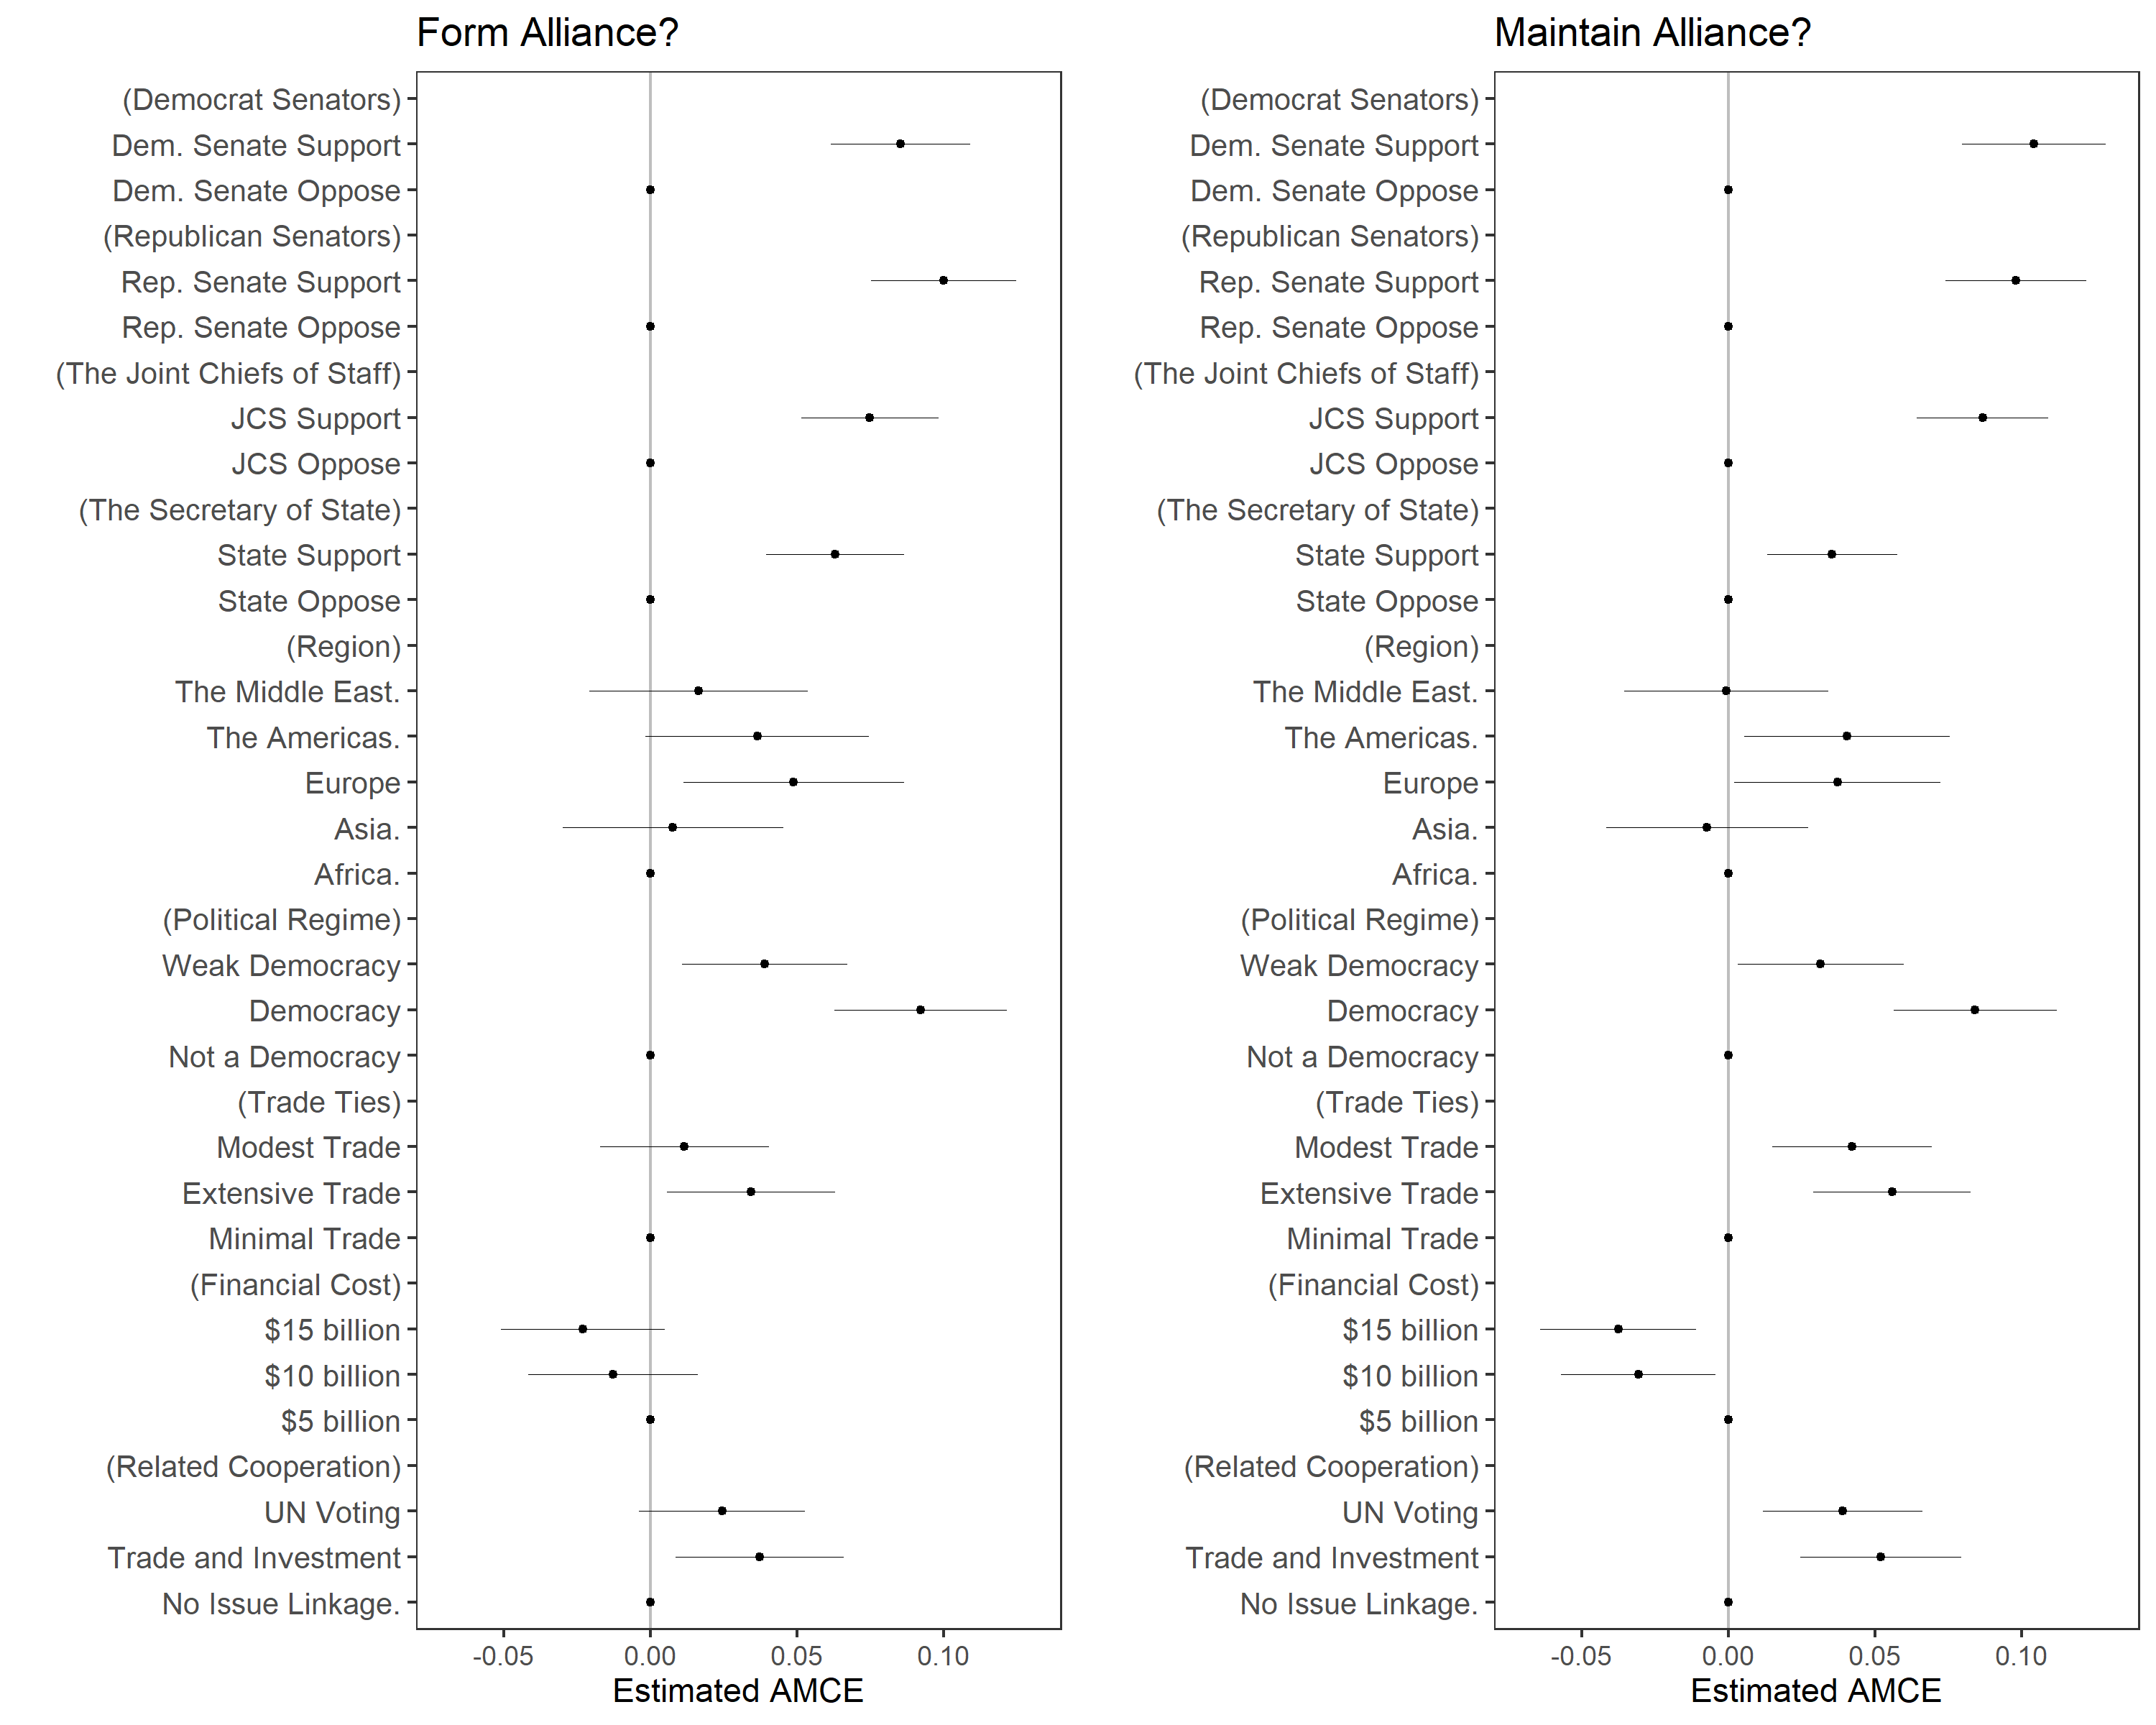
\includegraphics[width=0.95\textwidth]{../figures/joint-amce-plots.png}
	\caption{Average marginal component effect of elite cues and alliance characteristics on public support for forming or maintaining a hypothetical military alliance. Feature names in parentheses. Components marked with abbreviated labels and some attributes omitted to make the plot more legible.}
	\label{fig:joint-plot}
\end{figure}


Some alliance characteristics influence alliance attitudes as well. 
Allied regime type is particularly consequential. 
Established democracy increases support for alliance formation and maintenance.
The magnitude of the established democracy AMCE is comparable to elite cues.   
Weak democracies are marginally more likely than non-democracies to receive public support.


Issue linkages also encourage support for alliance formation and maintenance. 
Linkages to trade and investment with the United States increase support for alliance participation, relative to an alliance with no linkages. 
Political issue linkages in the United Nations bolster individual support, though this effect is smaller than that of trade. 
This adds a public opinion mechanism to prior findings that issue linkages can facilitate new alliance agreements \citep{Poast2012} and bolster alliance credibility \citep{Poast2013}. 


Last, alliance context and costs shift public attitudes. 
Trade ties and serious common threat encourage support for alliance maintenance. 
Relative to the lowest annual military spending cost, annual costs of \$10 billion or more decrease support for upholding an alliance.  
Respondents also view alliances in Europe or the Americas more favorably than commitments to African states. 


The above results assume that individuals respond in the same way to different cues and alliance characteristics. 
But individual concerns, especially the confluence of partisanship and foreign dispositions, structure foreign policy attitudes.
Examining how these factors change individual responses shows who elites lead.  



\subsection{Partisanship, Hawkishness, Isolationism, and Alliance Attitudes}



In this section, I estimate support for alliances across respondents with different partisan affiliations and foreign policy dispositions.  
This analysis helps establish who leads in public opinion towards alliances. 
If elite cues exert little impact or only push respondents in ways that match their predispositions, elites are more likely to follow public opinion. 
On the other hand, if elite cues change attitudes regardless of foreign policy dispositions, elites lead. 


In the following, I plot the marginal means of support for alliance participation for distinct foreign policy dispositions within the two major parties.  
The first pair of figures summarizes the overall average and marginal means of support given different elite cues. 
I then examine how respondents with different partisan affiliations and foreign policy dispositions view key alliance characteristics. 


\subsubsection{Elite Cues}


\autoref{fig:party-dispo-form-el} and \autoref{fig:party-dispo-main-el} show the marginal means of support for alliance formation and maintenance from elite cues across partisan and foreign policy disposition subgroups.\footnote{See the appendix for details on the distribution of foreign policy dispositions across party identification.} 
Each panel plots the marginal mean of support for each alliance attribute within every categorical combination of militant assertiveness, internationalism, and partisanship.
In every panel, a solid vertical line marks a marginal mean of .5 and a dashed line summarizes the baseline or average alliance choice across all attributes and levels.  
Both figures show how individuals in each group respond to elite cues. 


Alliance attitudes and responses to elite cues reflect a complex combination of foreign policy dispositions and partisanship. 
The same foreign policy dispositions have distinct implications for alliance attitudes among Republicans and Democrats, so partisanship matters.
At the same time, foreign policy dispositions produce substantial differences in alliance attitudes within parties.  


\begin{figure}[htpb]
	\centering
		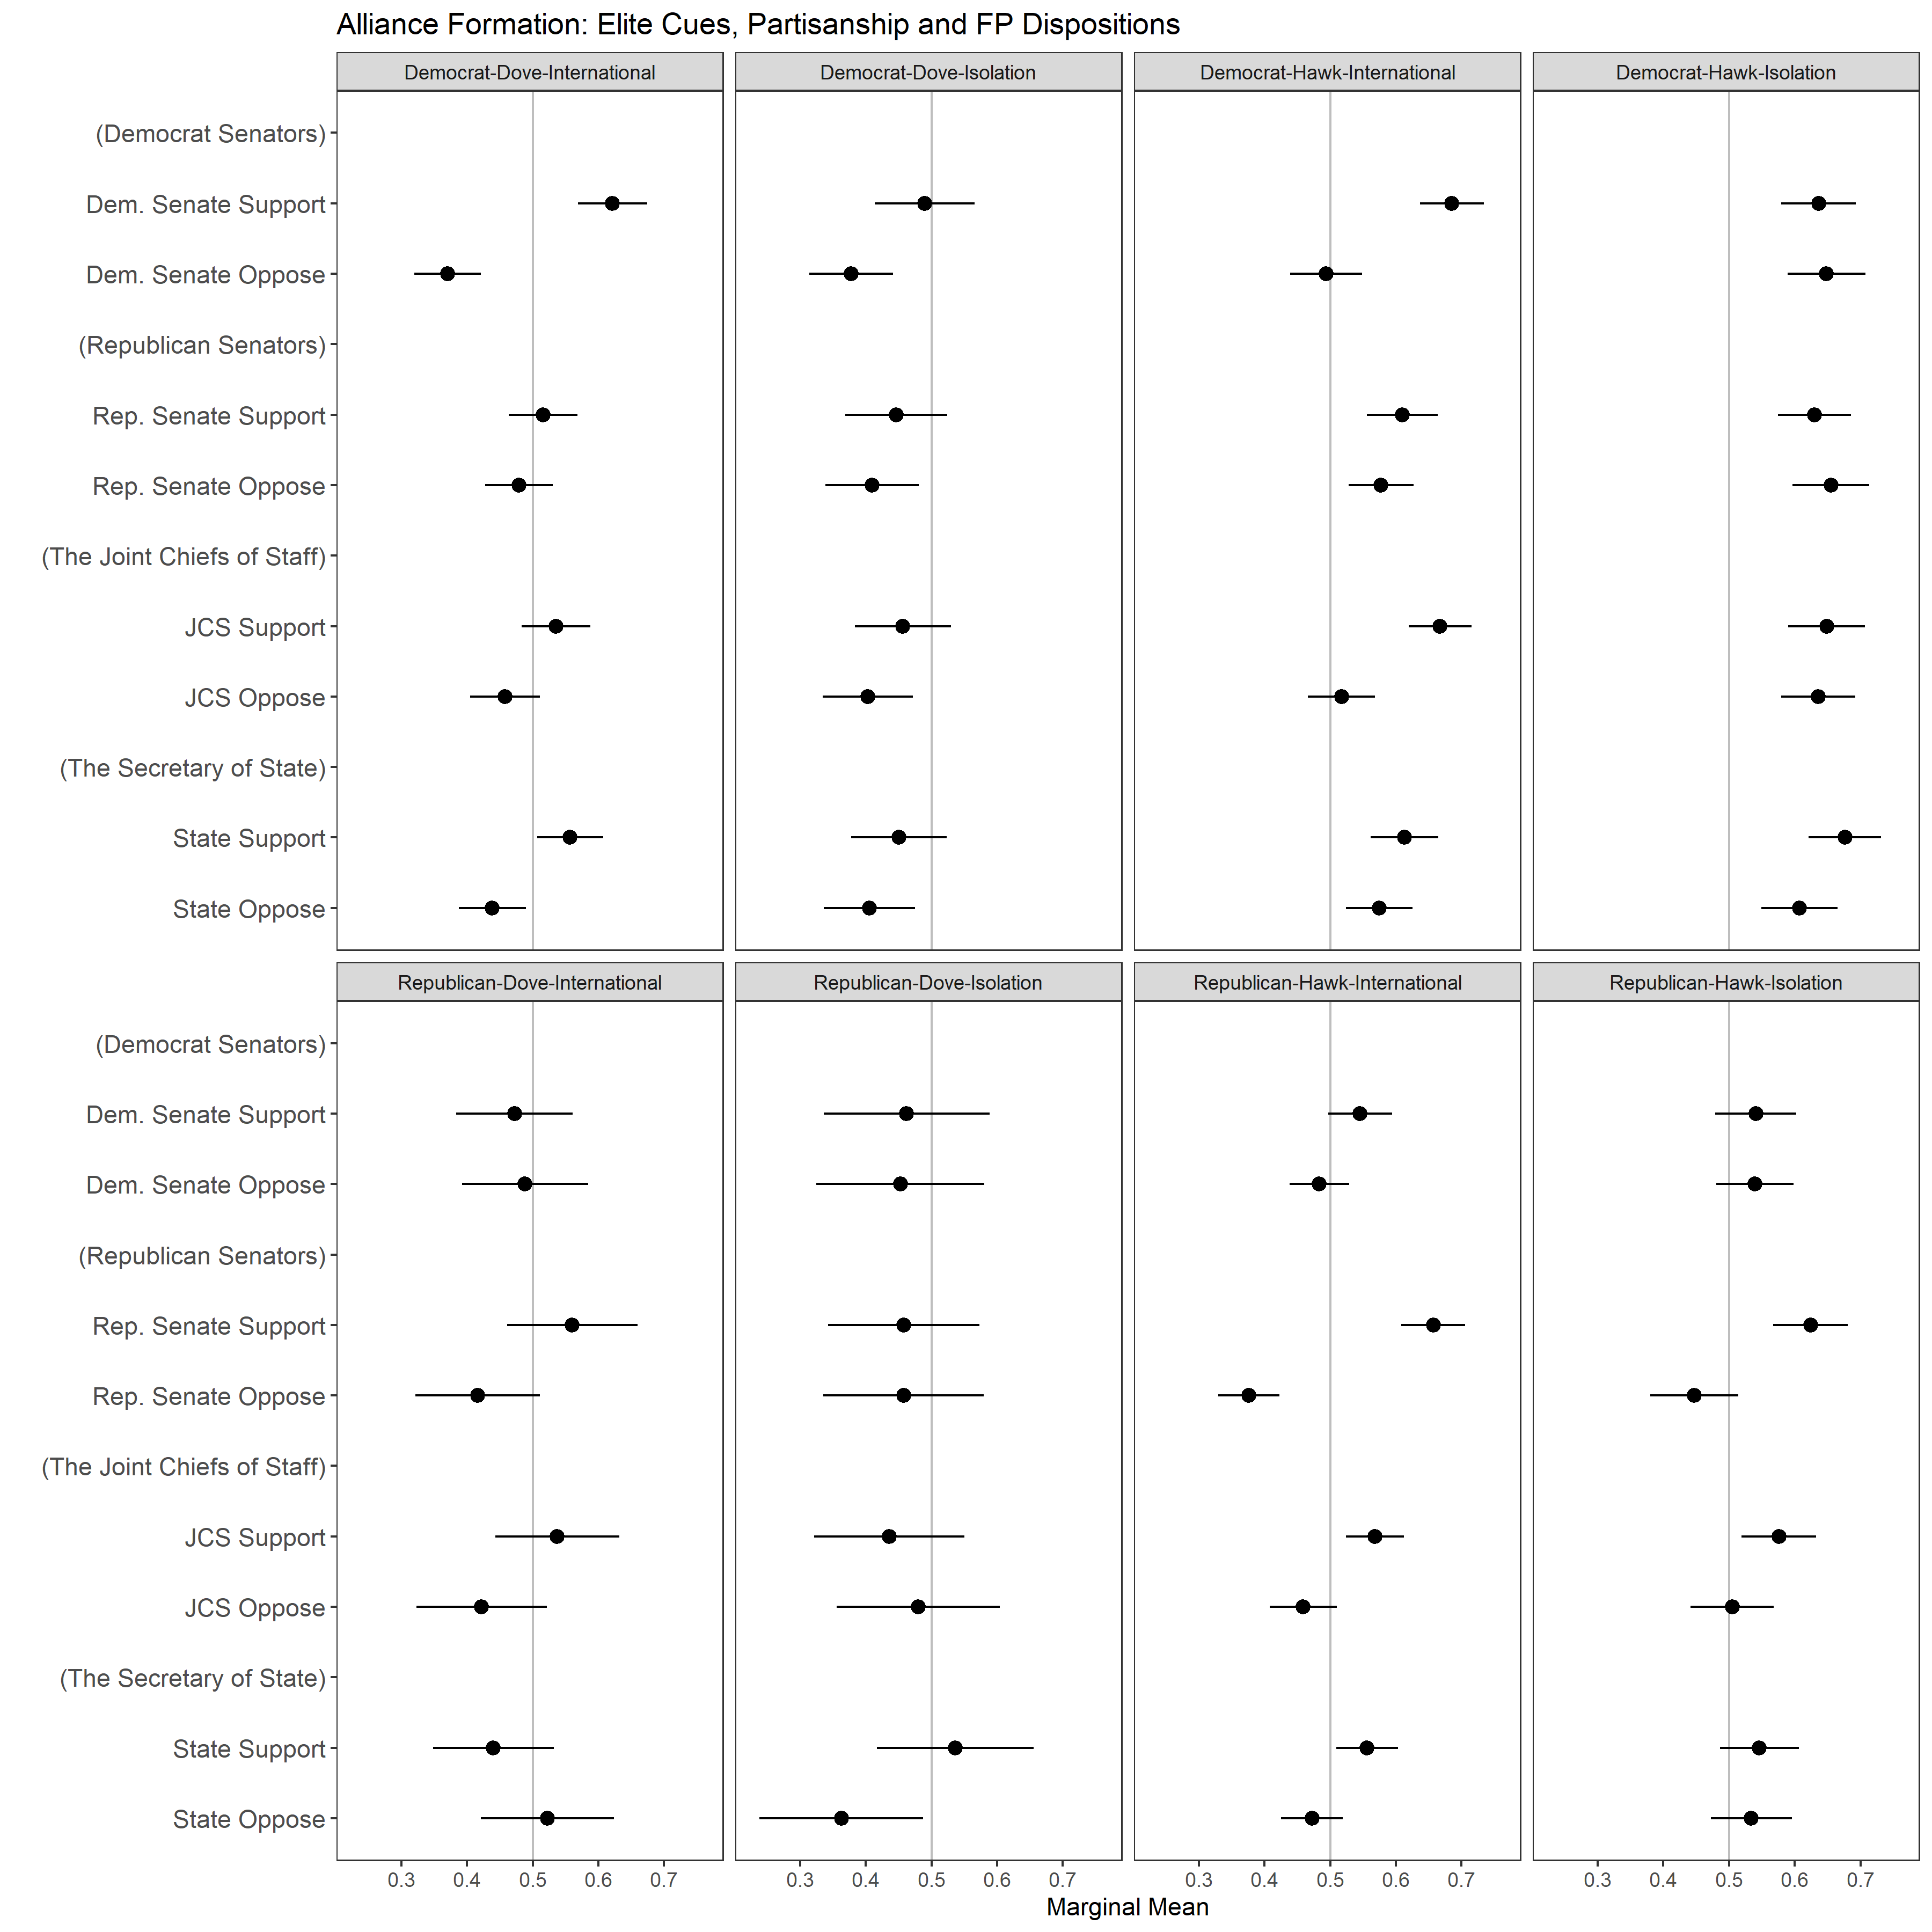
\includegraphics[width=0.95\textwidth]{../figures/party-dispo-form-el.png}
	\caption{Marginal means of support for forming hypothetical alliances across party identification and foreign policy dispositions given different elite cues. For each group, the estimates mark the marginal mean of support for alliance participation under different alliance treatments. The solid vertical line marks a marginal mean of .5, while the dashed line marks the average choice across all levels. Components marked with abbreviated labels to make the plot more legible. Independents omitted.}
	\label{fig:party-dispo-form-el}
\end{figure}


Among Democrats and Republicans, hawkishness increases support for alliance participation. 
There are partisan differences in this relationship, however, as hawkish Democrats express higher support for alliance participation than hawkish Republicans. 
Hawkish and isolationist Democrats are the strongest supporters of alliance participation. 
Hawkishness also increases support for alliance participation among isolationists. 


Isolationism alone does not reduce support for alliance participation.
Rather, alliance opposition comes from skeptics of international engagement and using force. 
Isolationist and dovish individuals are the greatest skeptics of alliance formation and maintenance. 
The combination of isolationism and limited support for military force is at the heart of alliance opposition. 
Although Republican doves are rare, they are integral to alliance skepticism in the GOP. 
Dovish Democrats are also more likely to oppose alliance participation.  


\begin{figure}
	\centering
		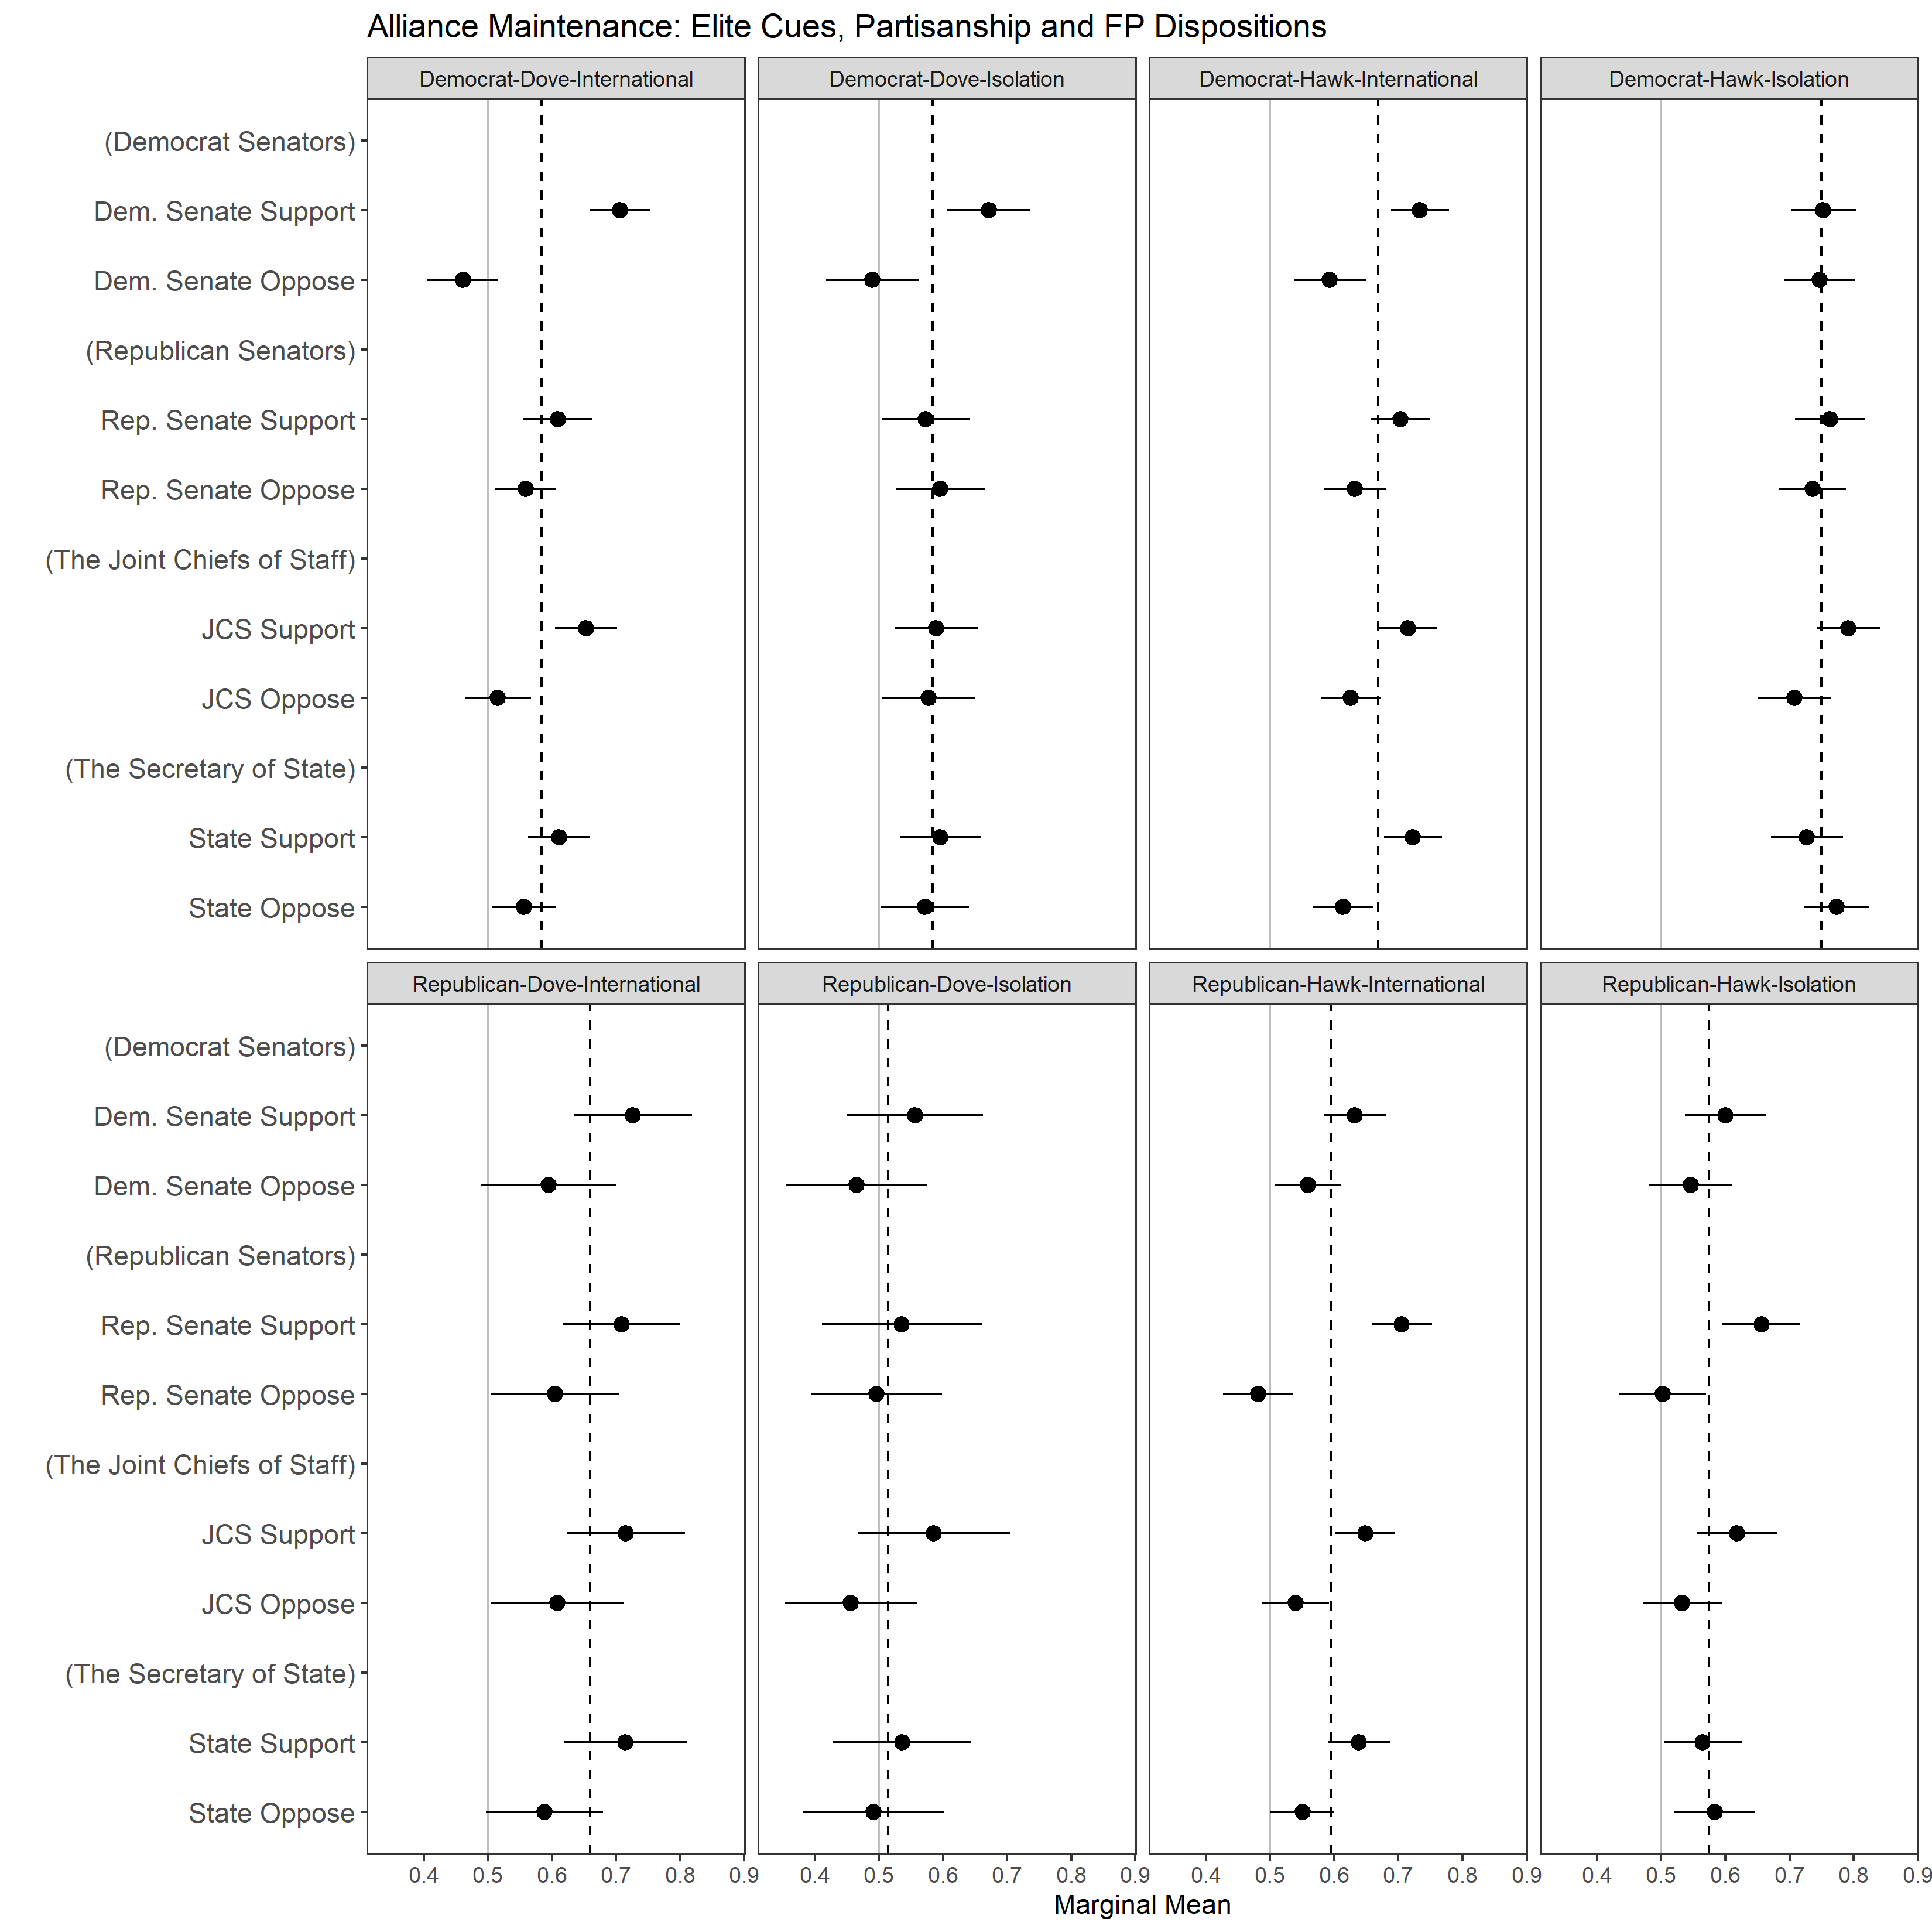
\includegraphics[width=0.95\textwidth]{../figures/party-dispo-main-el.png}
	\caption{Marginal means of support for maintaining hypothetical alliances across party identification and foreign policy dispositions given different elite cues. For each group, the estimates mark the marginal mean of support for alliance participation under different alliance treatments. The solid vertical line marks a marginal mean of .5, while the dashed line marks the average choice across all levels. Components marked with abbreviated labels to make the plot more legible. Independents omitted.}
	\label{fig:party-dispo-main-el}
\end{figure}


In addition to shifting baseline alliance attitudes, foreign policy dispositions change individual responses to elite cues. 
Isolationists are less likely to heed elite cues. 
Internationalist Democrats respond strongly to support from Democratic Senators, and also look to cues from the Secretary of State and Joint Chiefs of Staff. 
Hawkish and isolationist Democrats express consistent support for forming and maintaining alliances, albeit with some attention to military elite cues. 
The strongest alliance supporters in the Democratic party thus hold rigid alliance attitudes.


Among Republicans, hawks are most receptive to elite cues. 
Regardless of their view of international engagement, there are clear differences in alliance support for hawkish Republicans based on Republican Senate support or opposition.
Hawkish Republicans also follow cues from military elites, and internationalist hawks in the GOP pay further attention to diplomatic elites. 
As a result, Republican elites can lead alliance attitudes among individuals who are disposed to support forceful international engagement and thereby constrain alliance support among the most likely alliance backers in their party. 
The gap in hawkish Republican attitudes from differences in Republican elite support is especially pronounced in the alliance formation experiment. 
Dovish and isolationist Republicans pay little attention to elite cues. 
In the reverse of the Democratic party, the most likely alliance supporters in the Republican party hold more plastic alliance attitudes. 




% highlight differences in formation and maintenace
Individuals hold distinct attitudes towards alliance formation and maintenance. 
Forming new alliances has lower baseline support than maintaining existing treaties, so elite cues are crucial for new alliances. 
Only hawkish Democrats express clear support for alliance formation--- other respondents are divided or oppose new treaties.
Dovish isolationists dislike new alliances, though elites can persuade Democrats with this disposition. 
Whether elites support or oppose an alliance determines whether it has majority or minority support within each party. 


Alliance maintenance commands more robust support. 
Regardless of alliance characteristics or elite cues, the overall average and marginal means of support for alliance maintenance are almost all above .5. 
Even dovish isolationists in the GOP express a split verdict on alliance maintenance on average.


% wrap up
These results suggest that elite cues, partisanship and foreign policy dispositions interact to shape alliance attitudes.
Partisanship and foreign policy dispositions set the bases from which elite cues lead most of the public. 
There is an important partisan asymmetry in alliance attitudes as well. 
Democrat leaders can lead alliance skeptics and have less influence over the most committed alliance supporters. 
Republican elites lead alliance supporters, but cannot persuade committed alliance skeptics. 
As a result, elite cues exert substantial influence on most individuals in both parties, but elite influence depends on foreign policy dispositions. 


An online appendix provides further support for these results. 
In the appendix, I examine marginal means by partisanship and foreign policy dispositions alone, analyze responses to an open-ended question, and compare results with the continuous rating measure of alliances to inferences from the choice question.
All these checks are consistent with these findings. 


\section{Discussion and Conclusion} 


% Overview
I find that elites often lead public alliance attitudes, though how alliance attitudes change depends on where they start.  
Individuals follow cues from co-partisan elites, but their exact response depends on partisanship, hawkishness and isolationism. 
Some individuals hold rigid alliance attitudes. 
Allied democracy, issue linkages, shared threat, financial cost and trade have noticeable impacts as well.  


% thus, net on puzzle
Elites have substantial latitude to lead public opinion on alliances, but foreign policy dispositions constrain their influence. 
The most committed alliance supporters ---hawkish isolationist Democrats--- pay little attention to elite cues.
Similarly, elite cues have no impact on the most committed alliance skeptics --- dovish and isolationist Republicans. 
The result is a partisan gap in elite leadership of alliance attitudes. 
Republicans can lead copartisan alliance supporters, while Democrats can lead copartisan alliance skeptics. 


% bring it in on observed alliances
These findings have four implications for understanding public attitudes towards U.S. alliances like NATO. 
First, the Republican and Democratic parties have cores of committed alliance skeptics and supporters, respectively.
Outside these groups and independents, most Americans follow elite cues in forming alliance attitudes. 
This makes whether elites follow fixed alliance attitudes in their party a critical issue, because it could polarize the electorate.  


Second, my findings support the view that elite-driven public opinion cycles could make democratic commitments less reliable \citep{GartzkeGleditsch2004}. 
Although the results suggest that many members of the public hold considered opinions \citep{PageShapiro1992}, they also show substantial elite influence. 
Elite opposition rarely pushes alliance attitudes into majority opposition to existing treaties, but one set of elite cues can reduce aggregate support in both major parties.
In the Republican Party, elite opposition creates an even split in alliance maintenance attitudes. 
Negative cues from military or diplomatic elites would also bolster the impact of skeptical politicians and cut public support. 


Third, allied democracy reinforces public support for alliances.
Individuals in both parties prefer alliances with democracies. 
Democratic backsliding in U.S. allies could therefore undermine public support for alliances, especially by giving skeptical elites a powerful angle for criticism. 


% why NATO robust under Trump? 
Finally, these results help us understand public opinion towards alliances like NATO during the Trump administration.
Although Trump often criticized U.S. allies, alliance commitments usually commanded majority support throughout his administration \citep{PewNATO2020}. 
The relative stability of alliance attitudes reflects Democrats' aversion to Trump, allied democracy, countervailing cues from other elites and high baseline support for existing alliances. 
For many Republicans, hawkishness offsets isolationism in alliance attitudes.
Although Trump likely increased Republican skepticism of alliances, concern that he would inspire resurgent isolationism in the Republican party may have been overstated.
Isolationist and dovish Republicans did not change their alliance attitudes in response to Trump, as his rhetoric matched their views. 


% limitations
These findings have some limitations. 
For one, while the sheer variety of alliances means that the above profiles are plausible, generalizing from survey experiments is challenging. 
The artificial nature of a survey experiment provides essential control to disentangle public attitudes, but no hypothetical alliance can fully reflect real world commitments.


% can't show pandering
While this paper provides new insight into the question of who leads and who follows, it does not give a comprehensive account of the issue. 
How much and when elites decide to follow fixed alliance attitudes in their party falls outside the scope of this paper. 
Having identified who elites can lead, understanding the long-run dynamics of leading and following is a crucial subject for future research. 


% non-us results- might be different, subject for future inquiry
This study also focuses on the United States, which has an unusual alliance network. 
Though public opinion towards alliances in the United States is important, attitudes in other countries matter as well. 
Future research should examine the sources of alliance attitudes in other countries. 


% future stuff: feedback, content of elite cues
These results provide a foundation for further inquiry into the domestic politics of military alliances. 
Two questions are especially interesting in this respect.
First, how much feedback takes place between public opinion and elite cues? 
When do politicians follow rigid alliance attitudes or lead in a competing direction? 
Politicians might view marginal opinion shifts due to threat or allied democracy changes as an opportunity to encourage or arrest further changes in public support.
Second, would leaders face significant public disapproval if they withdrew from an alliance? 
This study focused on generic support, but future research should build on \citet{TomzWeeks2021} and examine specific alliance policy changes. 


These questions address how elites form and maintain domestic coalitions around international engagement. 
In the 75 years since the end of World War II, shifting elite cues, partisanship, generational experiences and allied characteristics may mean different groups back alliances today than in 1950. 
Tracking changes in the domestic coalitions backing alliances is another worthwhile task for future research.


% wrap it up 
In conclusion, public opinion towards alliances is largely a function of elite cues, but elites do not lead the whole electorate.  
Subsets of both parties hold rigid alliance attitudes. 
Alliances attitudes are therefore a complex mixture of elite cues and individual considerations. 



\newpage

% Bibliography
 
\bibliography{../../MasterBibliography} 




\end{document}
